\section{Belief Propagation} \label{BP}

The Warning Propagation algorithm is able to solve the decision problem and to compute valid assignments of SAT formulas. A different message passing method called the \emph{Belief Propagation} algorithm is able to determine the actual number of satisfying assignments and the fraction of those assignments where variables are restricted to fixed values. 

The messages sent in the BP algorithm are conditional probabilities $\mu \in [0, 1]$. The corresponding events are taken from the probability space built by all configurations $X$ of the  boolean variables $x_1, \ldots, x_n$. The used probability measure is a uniform distribution so for a SAT formula over $n$ variables each configuration has probability $P(X) = 2^{-n}$. \newline
This probability space can be restricted to only those configurations that satisfy a boolean formula $\mathcal{F}$. If there are $\mathcal{N} > 0$ satisfying assignments this conditioned probability measure factorizes to $$P(X \; | \; X \text{ satisfies } \mathcal{F}) = \mathcal{N}^{-1} \prod_{a \in A} f_a(X)$$
where $A$ is the set of clauses in $\mathcal{F}$ and $f_a(X)$ the characteristic function of a clause $a$ which is $1$ if $X$ satisfies $a$ and $0$ if not. \newline
The fraction of satisfying assignments where for example $x_1 = 1$ or $x_4 = 0$ can now be viewed as a marginal of the factorized function. \newline

In general, belief propagation is a message passing technique for approximating marginals of factorized probability distributions. In this chapter the BP equations and their interpretations in the SAT context are explained and demonstrated on an example formula.

\subsection{Propagation Algorithm} \label{BPA}

The basic procedure of sending and updating messages between nodes of the function's factor graph stays the same as in WP. Instead of warnings, the BP messages are conditional probabilities. From the converged probabilities one can obtain marginals and the function's normalization constant $\mathcal{N}$. With this information one gets the total number of satisfying assignments as well as the number of assignments where a single variable has a fixed value.

\subsubsection{Messages}
%The general idea behind Belief Propagation is to compute for each edge $u \rightarrow v$ a marginal 

The message $\mu_{a \rightarrow i}(x_i)$ sent from a factor $a$ to a variable $i$ is meant to be the probability that $a$ and all the factors behind $a$ are satisfied conditioned on $i$ taking the value $x_i$. 

%$\tau_{a \rightarrow i}$ is satisfied conditioned on $i$ taking the value $x_i$. 

The message $\mu_{i \rightarrow a}(x_i)$ sent in the opposite direction is the probability that $i$ takes the value $x_i$ in an assignment that satisfies $\tau_{i \rightarrow a}$.

\begin{example}
Let $\mathcal{F} = \underbrace{(x_1 \lor x_2 \lor \overline{x_3})}_a  \land \underbrace{(x_3 \lor x_4)}_b $.

\begin{figure}[h]
\centering

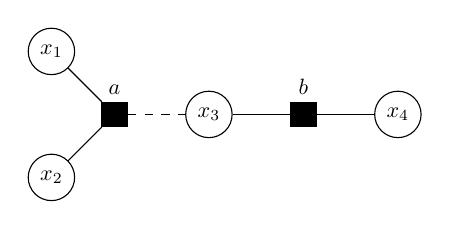
\begin{tikzpicture}[scale=0.8,transform shape]
   	\node[rectangle,draw=black, label = {$a$}, fill] (a) at (1,0) {$a$};
   	\node[rectangle,draw=black, label = {$b$}, fill] (b) at (4,0) {$a$};   
  \node[shape=circle,draw=black] (x1) at (0, 1) {$x_1$};
   
  \node[shape=circle,draw=black] (x2) at (0,-1) {$x_2$};
  \node[shape=circle,draw=black] (x3) at (2.5,0) {$x_3$};
  \node[shape=circle,draw=black] (x4) at (5.5,0) {$x_4$};
 


    
	\draw[-] (a) edge [right] node {} (x1);
	\draw[-] (a) edge [right] node {} (x2);
	\draw[-, dashed] (a) edge [right] node {} (x3);
	\draw[-] (b) edge [right] node {} (x3);
	\draw[-] (b) edge [right] node {} (x4);


\end{tikzpicture}
\end{figure}
The messages exchanged between $b$ and $x_3$ can be computed using only the definition: \newline
For example $\mu_{b \rightarrow 3}(1)$ is the probability that $(x_3 \lor x_4)$ is satisfied by an assignment where $x_3 = 1$. Its value is $1$ because each such assignment satisfies $b$. If $x_3 = 0$ however, only those assignments where $x_4 = 1$ will satisfy $b$ so $\mu_{b \rightarrow 3}(0) = 0.5$. \newline
Out of all 14 configurations satisfying $(x_1 \lor x_2 \lor \overline{x_3})$ there are $8$ where $x_3 = 0$ and $6$ where $x_3 = 1$, so $\mu_{3 \rightarrow b}(0) = \frac{4}{7}, \, \mu_{3 \rightarrow b}(1) = \frac{3}{7}$.
\end{example}

This method of counting desired configurations in the whole configuration space is infeasible for larger graphs. Instead the probabilities are obtained by message passing.

\subsubsection{Update Rules}


\begin{wrapfigure}{r}{0.3\textwidth}

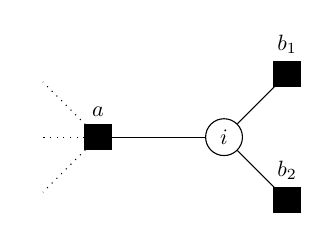
\begin{tikzpicture}[scale=0.8,transform shape]
   	\node[rectangle,draw=black, label = {$a$}, fill] (a) at (0,0) {$a$};
   	
\node[shape=circle,draw=black] (i) at (2,0) {$i$};   	
   	
   	\node[rectangle,draw=black, label = {$b_1$}, fill] (b1) at (3,1) {$a$};
   	\node[rectangle,draw=black, label = {$b_2$}, fill] (b2) at (3,-1) {$a$};

	\node[] (x1) at (-1,0) {};
	\node[] (x2) at (-1,1) {};
	\node[] (x3) at (-1,-1) {};

    \draw[dotted] (a) edge [right] node {} (x1);
    \draw[dotted] (a) edge [right] node {} (x2);
    \draw[dotted] (a) edge [right] node {} (x3);
	\draw[-] (a) edge [right] node {} (i);
	\draw[-] (i) edge [right] node {} (b1);
	\draw[-] (i) edge [right] node {} (b2);

\end{tikzpicture}
\end{wrapfigure}
$\mu_{i \rightarrow a}(x)$, the message passed to $a$, tells the probability that $i$ is $x_i = x$ considering only the factors on $i$'s side of the graph. \newline The node $i$ receives information about these factors through its neighbour vertices $b_i \neq a$. The incoming messages $\mu_{b_i \rightarrow i}(x)$ tell, if the factors are satisfied conditioned on $x_i = x$. \newline
Using Bayes' theorem and the fact that the messages $\mu_{b_i \rightarrow i}$ are conditionally independent, one can write the outgoing message  as a product of the incoming ones:
\begin{align*}
\mu_{i\rightarrow a}(x) = P(x_i = x \; | \; \tau_{i \rightarrow a} \text{ is sat.})
&= \frac{P(x_i = x) P(x_i = x \; | \; \tau_{i \rightarrow a} \text{ is sat.})}{P(\tau_{i \rightarrow a} \text{ is sat.})} \\
&= \underbrace{\frac{P(x_i = x)}{P(\tau_{i \rightarrow a}\text{ is sat.})}}_{C_{i \rightarrow a}} \prod_{b \neq a} \mu_{b \rightarrow i}(x) \\
\end{align*}
The factor $C_{i \rightarrow a}$ is the same for $x=0$ and $x=1$ so it suffices to compute the products for $x_i = 0$ and $x_i = 1$ and then to normalize so that $\mu_{i\rightarrow a}(0) + \mu_{i \rightarrow a}(1) = 1$. The usual notation to indicate the implicit existence of a normalization factor is $\mu_{i \rightarrow a}(x) \propto \prod \mu_{b \rightarrow i}(x)$ (\cite{lecture}). 

\begin{wrapfigure}{r}{0.3\textwidth}

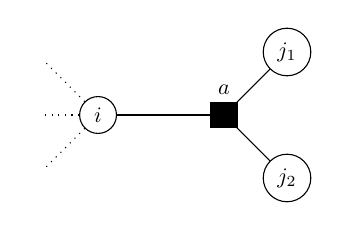
\begin{tikzpicture}[scale=0.8,transform shape]
   	\node[rectangle,draw=black, label = {$a$}, fill] (a) at (2,0) {$a$};
   	
\node[shape=circle,draw=black] (i) at (0,0) {$i$};   	
   	
   	\node[shape=circle,draw=black] (b1) at (3,1) {$j_1$};
   	\node[shape=circle,draw=black] (b2) at (3,-1) {$j_2$};

	\node[] (x1) at (-1,0) {};
	\node[] (x2) at (-1,1) {};
	\node[] (x3) at (-1,-1) {};

    \draw[dotted] (i) edge [right] node {} (x1);
    \draw[dotted] (i) edge [right] node {} (x2);
    \draw[dotted] (i) edge [right] node {} (x3);
	\draw[-] (a) edge [right] node {} (i);
	\draw[-] (a) edge [right] node {} (b1);
	\draw[-] (a) edge [right] node {} (b2);

\end{tikzpicture}
\end{wrapfigure}

To compute $\mu_{a \rightarrow i}(x)$ one has to sum over all configurations $X$ of the variables in $a$ where $x_i = x$. If a configuration does not satisfy $a$, it contributes nothing to $\mu_{a \rightarrow i}(x_i)$. If it does, one has to compute the probability that it also satisfies the other factors in $\tau_{a \rightarrow i}$. The probability that a configuration where $j$ takes the value $x_j$ satisfies the factors behind the neighbour variable $j$ is $\mu_{j \rightarrow a}(x_j)$. Again these probabilities are independent and the probability for all factors is simply the product.

$$\mu_{a \rightarrow i}(x_i) = \sum_{ \sim \{x_i\}} f_a(X) \prod_{j \neq i} \mu_{j \rightarrow a}(x_j)$$

The expression $\sim\{x_i\}$ means that the sum goes over all possible configurations $X$ of $a$'s variables with the exception of the value of $x_i$ which is always the same. 
\begin{example}
Now the messages from the first example can be computed with belief propagation.
% $$\mathcal{F} = \underbrace{(x_1 \lor x_2 \lor \overline{x_3})}_a  \land \underbrace{(x_3 \lor x_4)}_b $$
Since the formula's factor graph is a tree, the updates can be scheduled so that each message has to be computed only once.

\begin{itemize}
\item Level 0 (Leaves)

The leaves are all variable nodes. As they receive no incoming messages they will all send the same constant message. The empty product in the update rule evaluates to $1$, after normalization the values are \newline $\mu_{1 \rightarrow a}(0) = \mu_{1 \rightarrow a}(1) = 1/2$. The same holds for $2 \rightarrow a$ and $4 \rightarrow b$.

\item Level 1.
The message of level $1$ are both sent from factors to variables: 
\begin{align*}
\mu_{a \rightarrow 3}(0) = &\mu_{1 \rightarrow a}(0)\mu_{2 \rightarrow a}(0) + \mu_{1 \rightarrow a}(0)\mu_{2 \rightarrow a}(1) + \mu_{1 \rightarrow a}(1) \mu_{2 \rightarrow a}(0) \\ + & \mu_{1 \rightarrow a}(1)\mu_{2 \rightarrow a}(1) = 1 \\
\mu_{a \rightarrow 3}(1) = &\mu_{1 \rightarrow a}(0)\mu_{2 \rightarrow a}(1) + \mu_{1 \rightarrow a}(1) \mu_{2 \rightarrow a}(0) + \mu_{1 \rightarrow a}(1)\mu_{2 \rightarrow a}(1) \\ = &3/4 \\
\mu_{b \rightarrow 3}(0) = &\mu_{4 \rightarrow b}(1) = 1/2 \\
\mu_{b \rightarrow 3}(1) = &\mu_{4 \rightarrow b}(0) + \mu_{4 \rightarrow b}(1) = 1
\end{align*}

\item Level 2.
The unnormalized values for $3 \rightarrow b$ are $0.5$ and $1$. After normalization one gets $\mu_{3 \rightarrow b}(0) = \frac{0.5}{0.5 + 1} = \frac{1}{3}$ and $\mu_{3 \rightarrow b}(1) = \frac{2}{3}$. \newline
The values $\mu_{3 \rightarrow a}(0) = \frac{1}{1 + 0.75} = \frac{4}{7}$ and $\mu_{4 \rightarrow a}(1) = \frac{3}{7}$ are obtained in the same way.
%  \item Level 3

\end{itemize}
The values for the remaining 3 edges of level $4$ can be looked up in the tabular

\end{example}

\begin{figure}[h]
\begin{floatrow}
\centerfloat
\capbtabbox{%
  \begin{tabular}{ccc} \hline
  Edge & $\mu(0)$ & $\mu(1)$ \\ \hline
  $1 \rightarrow a$ & $1/2$ & $1/2$ \\
  $2 \rightarrow a$ & $1/2$ & $1/2$ \\ 
  $4 \rightarrow b$ & $1/2$ & $1/2$ \\ 
  $a \rightarrow 3$ & $1$   & $3/4$ \\ 
  $b \rightarrow 3$ & $0.5$ & $1$ \\ 
  $3 \rightarrow a$ & $1/3$ & $2/3$ \\ 
  $3 \rightarrow b$ & $3/7$ & $4/7$ \\ 
  $a \rightarrow 2$ & $5/6$ & $1$ \\ 
  $a \rightarrow 1$ & $1$ & $5/6$ \\ 
  $b \rightarrow 4$ & $4/7$ & $1$ \\ 
  \end{tabular}
}{}
%{%
%  \caption{A table}%
%}
\ffigbox{%
  \centering
  \centerfloat
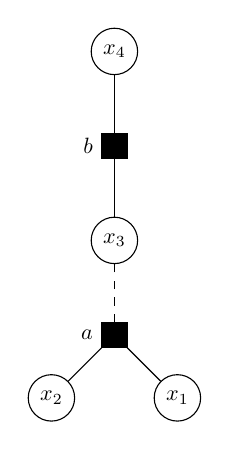
\begin{tikzpicture}[scale=0.8,transform shape]
   	\node[rectangle,draw=black, label = left:{$a$}, fill] (a) at (0,1) {$a$};
   	\node[rectangle,draw=black, label = left:{$b$}, fill] (b) at (0,4) {$a$};   
  \node[shape=circle,draw=black] (x1) at (1, 0) {$x_1$};
   
  \node[shape=circle,draw=black] (x2) at (-1,0) {$x_2$};
  \node[shape=circle,draw=black] (x3) at (0,2.5) {$x_3$};
  \node[shape=circle,draw=black] (x4) at (0,5.5) {$x_4$};
 


    
	\draw[-] (a) edge [right] node {} (x1);
	\draw[-] (a) edge [right] node {} (x2);
	\draw[-, dashed] (a) edge [right] node {} (x3);
	\draw[-] (b) edge [right] node {} (x3);
	\draw[-] (b) edge [right] node {} (x4);


\end{tikzpicture}


}{%
  %\caption{A figure}%
}
\end{floatrow}
\end{figure}


The equations described above are the general BP update rules that can be applied not only to SAT problems but to any problem that is solved by belief propagation.
In \cite{survprob} and \cite{lecture} these standard rules are expressed in a different, but equivalent way to make computation easier. \newline
Instead of computing functions where $\mu_{i \rightarrow a}(0)$ and $\mu_{i \rightarrow a}(1)$ add up to $1$, one can also compute the value $\gamma_{i \rightarrow a}$, the probability that $x_i$ violates $a$. 
It can be expressed as $\gamma_{i \rightarrow a} = \left\{
  \begin{array}{@{}ll@{}}
    \mu_{i \rightarrow a}(0) & \text{if}\ J_a^i = -1 \\
    \mu_{i \rightarrow a}(1), &  \text{if}\ J_a^i = 1
  \end{array}\right.$
  

In the original BP equation for $\mu_{a \rightarrow i}(x_i)$ one has to sum over all satisfying configurations of $a$'s variables $j \neq i$. Since there is only one configuration that does not satisfy $a$ it is easier to just compute the probability of this single configuration. The message $\delta_{a \rightarrow i}$ is the probability that all of $a$'s neighbours are in a state that violates $a$ (conditioned on $\tau_{a \rightarrow i}$ still being satisfiable). The probabilities for each $j$ to be in such a state are exactly the values of the incoming messages $\gamma_{j \rightarrow a}$ which are conditionally independent.
$\delta_{a \rightarrow i} = \prod_{j \neq i} \gamma_{j \rightarrow a}$ is the first update equation for the modified BP version.

The more complicated part is to compute $\gamma_{i \rightarrow a}$ from incoming messages $\delta_{b \rightarrow i}$. The probability that $i$ violates $a$ conditioned on $\tau_{i \rightarrow a}$ being satisfied is again proportional to the probability  that $\tau_{i \rightarrow a}$ is satisfied conditioned on $i$ violating $a$. This is the case exactly if no $b \neq a$ fixes $i$ to the value that would satisfy $a$.
$$\gamma_{i \rightarrow a} \propto P_{i \rightarrow a}^u := \prod_{b \in V_a^s(i)} (1 - \delta_{b \rightarrow i})$$
To get the real value of $\gamma_{i \rightarrow a}$ one has to normalize so that $P_{i \rightarrow a}^u$ and the probability for $i$ to satisfy $a$, $P_{i \rightarrow a}^s$, add up to $1$. \newline

With this this new formulation the messages can be obtained without summing over all possible configurations like in the last example and without summing over all possible configurations of a single variable's clauses like in the standard BP rules. \newline
The overall update procedure can now be described as

\begin{lstlisting}[mathescape=true, frame = single]
	Belief Propagation Algorithm
	  Input: A CNF formula and its factor graph
	0. Randomly initialize all message $\delta_{a \rightarrow i} \in_R [0, 1]$
	
	1. For $t=0$ to $t = t_{max}$
		1.1 Compute in random order for all edges (a, i)
		  $\delta_{a \rightarrow i} := \prod_{j \in V(a) \setminus i} \gamma_{j \rightarrow a}$		 
		where $\gamma_{j \rightarrow a} := \frac{P_{j\rightarrow a}^u}{P_{j\rightarrow a}^u + P_{j\rightarrow a}^s} = \frac{\prod_{b \in V_a^s(j)} (1 - \delta_{b \rightarrow j})}{\prod_{b \in V_a^s(j)} (1 - \delta_{b \rightarrow j}) + \prod_{b \in V_a^u(j)} (1 - \delta_{b \rightarrow j})}$
		 		
		1.2 If no $\delta_{a \rightarrow i}$ has changed more than $\epsilon$ goto 2.
	2. If $t = t_{max}$ return UN-CONVERGED, else return the generated warnings $\delta_{a \rightarrow i}^{\star}$
\end{lstlisting}

\subsection{Marginal Probabilities and Valid Assignments}

If the BP-Algorithm returns a set of converged messages one can obtain the single variable marginal $\mu_i = P(x_i = 1 \; | \mathcal{F} \text{ is satisfied})$ in the same way, the values $P_{i \rightarrow a}$ where defined: The normalized probability that $\mathcal{F}$ is satisfied conditioned on $x_i = 1$.
$$ \mu_i := \frac{\prod_{b \in V_-(i)} (1 - \delta^\star_{b \rightarrow i})}{\prod_{b \in V_-(i)} (1 - \delta^\star_{b \rightarrow i}) + \prod_{b \in V_+(i)} (1 - \delta^\star_{b \rightarrow i})}$$

At each step of the algorithm one can obtain in the same way the current \emph{belief} that $x_i = 1$ which has a changing value until the messages converge. $\mu_i$ is the final belief induced by the converged messages. \newline

These marginals are used to obtain satisfying assignments in the so called \emph{Belief Propagation Guided Decimation} algorithm. Like CID, the algorithm stepwise assigns  values to a formula's variables.

For each variable $i$ the BP algorithm is run and $x_i$ is set to $1$ with probability $\mu_i$ and to $0$ with probability $1 - \mu_i$. Then the graph is cleaned like in the CID algorithm and the next variable can be assigned. After assigning a value to $x_i$ the formula must still be satisfiable because $x_i$ will be set to a value with positive marginal which means there exist assignments in which $x_i$ takes exactly the chosen value. By induction the returned assignment is valid.

\begin{lstlisting}[mathescape=true, frame = single, escapechar=\%]
	Belief Propagation Guided Decimation %\cite{BPGuideMe}%
	  Input: A CNF formula and its factor graph
	  
	1. For $i = 1, \ldots, n$ do
		1.1 Run BP and compute $\mu_i$
		1.2 Assign $ \rho(x_i) = \left\{
  \begin{array}{@{}ll@{}}
    1 & \text{with probability } \mu_i \\
    0, &  \text{with probability } 1 - \mu_i 
  \end{array} \right.  $
	2. Return the complete assignment
\end{lstlisting}

For loopy graphs where the beliefs may be incorrect,  usually in each step the variable with the strongest belief (the variable $i$ that maximizes $|\mu_i|$) is assigned a value.

\begin{example}
In a final example, BPGD can be used to compute an assignment for the formula $\mathcal{F} = \underbrace{(x_1 \lor x_2 \lor \overline{x_3})}_a  \land \underbrace{(x_3 \lor x_4)}_b $
\begin{figure}[h]
\begin{floatrow}
\centerfloat
\capbtabbox{%
  \begin{tabular}{ccc} \hline
  Edge & $\gamma^\ast$ & $\delta^\ast$ \\ \hline
  $1 \rightarrow a$ & $1/2$  \\
  $2 \rightarrow a$ & $1/2$ \\ 
  $4 \rightarrow b$  &$1/2$ \\ 
  $a \rightarrow 3$ & &  $1/4$ \\ 
  $b \rightarrow 3$ & & $1/2$ \\ 
  $3 \rightarrow a$ & $2/3$  \\ 
  $3 \rightarrow b$ & $3/7$ \\ 
  $a \rightarrow 2$ & &$1/3$ \\ 
  $a \rightarrow 1$ & &$1/3$ \\ 
  $b \rightarrow 4$  & & $3/7$\\ 
  \end{tabular}
}{}
%{%
%  \caption{A table}%
%}
\ffigbox{%
  \centering
  \centerfloat
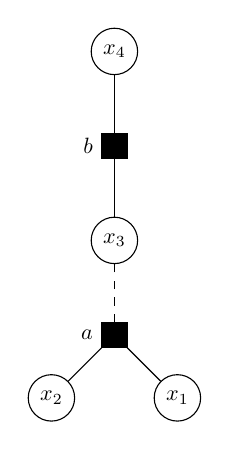
\begin{tikzpicture}[scale=0.8,transform shape]
   	\node[rectangle,draw=black, label = left:{$a$}, fill] (a) at (0,1) {$a$};
   	\node[rectangle,draw=black, label = left:{$b$}, fill] (b) at (0,4) {$a$};   
  \node[shape=circle,draw=black] (x1) at (1, 0) {$x_1$};
   
  \node[shape=circle,draw=black] (x2) at (-1,0) {$x_2$};
  \node[shape=circle,draw=black] (x3) at (0,2.5) {$x_3$};
  \node[shape=circle,draw=black] (x4) at (0,5.5) {$x_4$};
 


    
	\draw[-] (a) edge [right] node {} (x1);
	\draw[-] (a) edge [right] node {} (x2);
	\draw[-, dashed] (a) edge [right] node {} (x3);
	\draw[-] (b) edge [right] node {} (x3);
	\draw[-] (b) edge [right] node {} (x4);
\end{tikzpicture}


}{%
  %\caption{A figure}%
}
\end{floatrow}
\end{figure}


The beliefs $\mu_i$ are $\mu_1 = \frac{1}{1 + (1 - \delta^\ast_{a \rightarrow 1})} = 3/5$, $\mu_2 = \frac{1}{1 + (1 - \delta^\ast_{a \rightarrow 2})} = 3/5$, $\mu_3 = \frac{1  -\delta^\ast_{a \rightarrow 3}}{(1 - \delta^\ast_{a \rightarrow 3}) + (1 - \delta^\ast_{b \rightarrow 3})} = 3/5$ and $\mu_4 = \frac{1}{1 + (1 -  \delta^\ast_{b \rightarrow 4})} = 7/10$.

With probability $3/5$, $x_1$ is set to $1$ the and the cleaned formula is \newline $(x_3 \lor x_4)$ which can be solved recursively.
\end{example}